%% ---------------------------------------------------------------------------------------------------------------------

\chapter{\textit{go-geiger}: Identification of Unsafe Usage}\label{ch:go-geiger}

This chapter presents \toolGeiger{}, a tool to find usages of the \unsafe{} \acrshort{API} in Go packages and their
dependencies.
Furthermore, an empirical study on \unsafe{} usage in open-source projects using \toolGeiger{} is shown, and a novel
data set of labeled samples of \unsafe{} code is described.
Figure~\ref{fig:outline4} shows which parts of the contributions of this thesis are given in this chapter.

\begin{figure}[ht]
    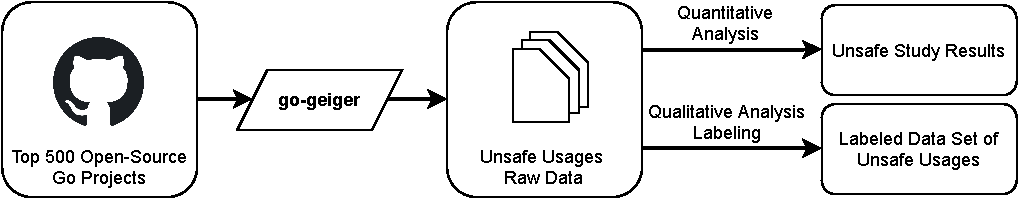
\includegraphics[width=\textwidth]{assets/figures/chapter4/outline4.pdf}
    \caption{Role of Chapter 4 in Thesis Outline}
    \label{fig:outline4}
\end{figure}



%% ---------------------------------------------------------------------------------------------------------------------

\section{Design}\label{sec:go-geiger:design}

The novel tool \toolGeiger{} is designed to identify usages of the \unsafe{} \acrshort{API} in Go source code.
In contrast to existing tools like \toolGosec{}, it includes the dependencies of Go packages in the analysis, which
gives a much better picture of possible \unsafe{} usages.
It is inspired by \toolCargoGeiger{}\footnote{\url{https://github.com/rust-secure-code/cargo-geiger}}, a similar tool
for detecting the use of unsafe code blocks in Rust programs.
Figure~\ref{fig:go-geiger-architecture} shows the architecture of \toolGeiger{}.

\begin{figure}[htp!]
    %\vspace{2mm}
    \centering
    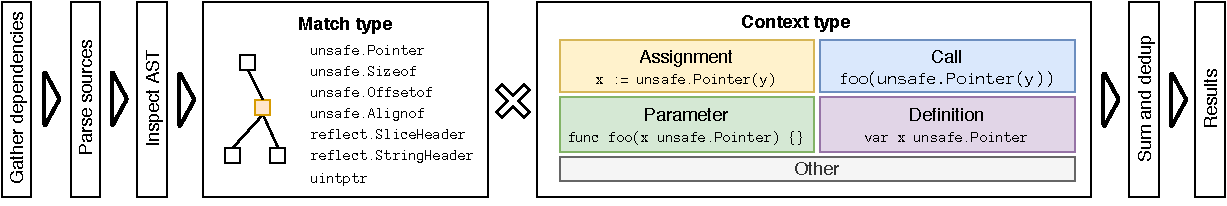
\includegraphics[width=\textwidth]{assets/figures/chapter4/go-geiger-architecture.pdf}
    \caption{Architecture of the \toolGeiger{} tool to detect unsafe usages}
    \label{fig:geiger-architecture}
    %\vspace{-10pt}
\end{figure}


First, the dependency tree of the packages that are given for analysis is built.
Then, the sources of all the packages in this tree are parsed, and the resulting abstract syntax tree (\acrshort{AST})
is inspected.
Within the \acrshort{AST}, usages of the \unsafe{} \acrshort{API} are identified.
Each usage is assigned a tuple of labels consisting of \textit{match type} and \textit{context type}.
The match type represents the part of the \unsafe{} \acrshort{API} that is used.
It can be either of the four \unsafe{} package members \textit{Pointer}, \textit{Sizeof}, \textit{Offsetof}, and
\textit{Alignof}, the \textit{reflect} package fields \textit{SliceHeader} and \textit{StringHeader}, or the
\textit{uintptr} keyword.
The context type indicates the functional part of code that the usage is found in.
It can be either an \textit{assignment}, a \textit{call} of a function, a function \textit{parameter} definition, or a
\textit{variable} definition.
If the context can not be assigned to one of these four options, then it is set to \textit{other}.
This context allows to filter the search for \unsafe{} usages to particular functional code positions.
There is a \toolGeiger{} command line parameter to request this filtering.
For example, it is possible to count only \unsafe{} usages that are used within parameters of function calls.
After the \unsafe{} usages are identified, they are counted.
For this, it is necessary to take care of package deduplication.
If a particular package exists in the dependency tree multiple times and is reachable on different paths, it must still
be counted only once when calculating the sum of \unsafe{} usages in a package's dependencies.
This is because the package does not get any less safe by including the same code multiple times, the code is already
part of the resulting program.
Finally, the analysis results are shown to the user.
It is possible to output the \unsafe{} usage counts as well as the lines of code containing the usages.

The source code and documentation of \toolGeiger{} is available on
\github{}\footnote{\url{https://github.com/jlauinger/go-geiger}}.
It can be installed using the standard Go \acrshort{CLI} tool.
To execute it, append the package names that should be checked as parameters.
For example, to examine a local package for \unsafe{} usages run \textit{go-geiger ./my/package}.
There is no limitation on the number of packages that can be supplied as parameters.
Figure~\ref{fig:go-geiger-screenshot} shows a screenshot of \toolGeiger{}.
It presents the analyis results for the \textit{go-geiger} source code itself.
The output is truncated is missing parts of the table with \unsafe{} counts, which have been excluded to decrease the
space needed to display the figure.

\begin{figure}[htp!]
    %\vspace{2mm}
    \centering
    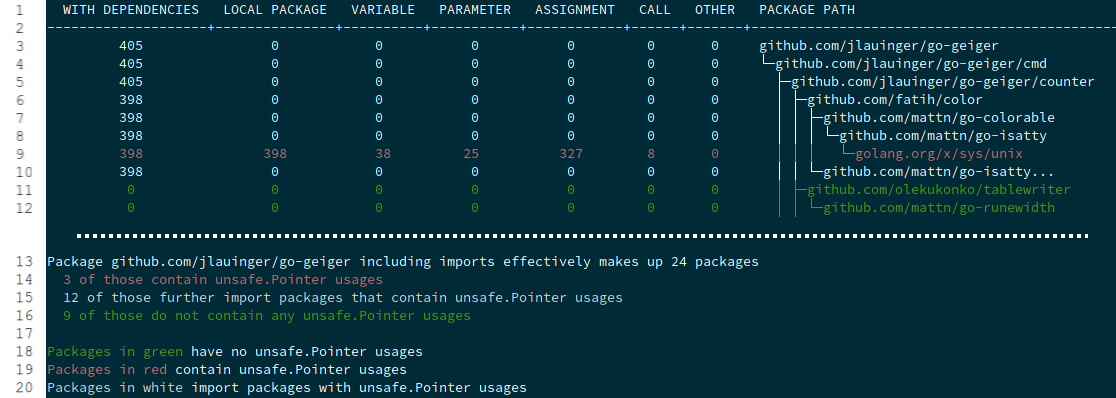
\includegraphics[width=\textwidth]{assets/images/chapter4/go-geiger-screenshot.png}
    \caption{Usage example screenshot of \toolGeiger{}}
    \label{fig:go-geiger-screenshot}
    %\vspace{-14pt}
\end{figure}


The output shown in Figure~\ref{fig:go-geiger-screenshot} is composed of three parts.
The first is a table showing the \unsafe{} usage counts for each package in the dependency tree for the packages
given for analysis.
The first column indicates the total number of usages in the package including all its dependencies.
The second column shows the number for the package alone, without the dependencies.
The heading for this column is \textit{local package}.
Next, there are five columns with individual usage counts for the four possible usage contexts described above,
\textit{variable}, \textit{parameter}, \textit{assignment}, \textit{call}, as well as \textit{other} for all matches
that could not be assigned to any of them.
These columns add up to the \textit{local package} count.
Finally, the import path for the package is given to identify it.
Lines that are printed in green (the last \checkNum{two} lines in Figure~\ref{fig:go-geiger-screenshot}) represent
packages with no local \unsafe{} usages.
Red lines (e.g. the \checkNum{seventh} line) are packages that directly contain \unsafe{} code, and white lines indicate
that the package does not contain \unsafe{} usages itself but instead introduces them through its dependencies.
After the table, there is a summary of the number of packages belonging into these three categories green, red, and
white, and finally a legend for the colors.


%% ---------------------------------------------------------------------------------------------------------------------

\section{Implementation}\label{sec:go-geiger:implementation}

The identification of the dependency tree for the packages to analyze, as well as the parsing of the source code is done
using the standard Go compiler toolchain.
It is accessable using the \textit{packages}
\acrshort{API}\footnote{\url{https://pkg.go.dev/golang.org/x/tools/go/packages}}.
Similarly, the inspection of the \acrshort{AST} is done using the \acrshort{API} available though the \textit{ast}
package in Go\footnote{\url{https://golang.org/pkg/go/ast/}}.

To find \unsafe{} usages corresponding to the different match types shown in Figure~\ref{fig:go-geiger-architecture},
the \acrshort{AST} is filtered for \textit{SelectorExpr} and \textit{Ident} nodes.
The first represent selector expressions, which indicate possible access of a member of another package, like in a usage
of \textit{unsafe.Pointer}.
The second is used to find instances of \textit{uintptr}.
In both cases the concrete identifier names in the \acrshort{AST} nodes are checked to distinguish \unsafe{} usages from
arbitrary other field accesses.
The context type is determined by going up in the \acrshort{AST} starting at the expression node corresponding to a
given \unsafe{} usage.
For example, an \unsafe{} usage is considered part of the \textit{assignment} context type if it is a descendent of
either an \textit{AssignStmt}, \textit{CompositeLit}, or \textit{ReturnStmt} node.
The \textit{call}, \textit{parameter}, and \textit{variable} classes correspond to \textit{CallExpr}, \textit{FuncDecl},
and \textit{GenDecl} nodes, respectively.
To achieve an effective assignment of the context type, the order in which the different types are checked is important.
This is because an \unsafe{} usage have reason to be included in several context types such as \textit{call} and
\textit{assignment} in an example like \textit{x := f(unsafe.Pointer(y))}.

The \unsafe{} usage counts are first collected for each package.
A cache is used to avoid analyzing the same package multiple times if it is present several times in the dependency
tree.
When the usage count including dependencies is calculated, \toolGeiger{} starts with the root packages that were
requested for analysis by the user, and recursively calculates the respective counts.
Again, the cache is used to avoid summing up multiple times.
This approach is a depth-first traversal of the dependency tree.

Automated acceptance testing verifies that \toolGeiger{} works as intended.
The test is done by running \toolGeiger{} on a test fixture package with a known number of \unsafe{} usages.
Then, the output is checked for the expected usage counts.


%% ---------------------------------------------------------------------------------------------------------------------

\section{Evaluation}\label{sec:go-geiger-evaluation}

To evaluate \toolGeiger{} on real-world code, it is used to gather empirical data about the usage of \unsafe{} in
popular open-source Go projects.
This section presents a study which was designed to answer the following research questions:

\begin{enumerate}[left=0.5cm, label={RQ\arabic*}]
    \item How prevalent is \unsafe{} in Go projects? \label{rq:prevalApp}
    \item How deep are \unsafe{} code packages buried in the dependency tree? \label{rq:depsDepth}
    \item Which \unsafe{} keywords are used most? \label{rq:distTypes}
    \item Is there a correlation between \unsafe{} usage and common project metrics such as age or popularity? \label{rq:popularity}
    \item How does the use of \unsafe{} change over time? \label{rq:changeTime}
    \item Does \toolGeiger{} provide additional insights into \unsafe{} usage compared to existing linter tools? \label{rq:linterComparison}
    \item Which \unsafe{} operations are used in practice, and for what purpose? \label{rq:purpose}
\end{enumerate}

The following subsections first discuss how the data for this study was gathered and then answer research
questions~\ref{rq:prevalApp} to~\ref{rq:linterComparison}.
Then, Section~\ref{sec:go-geiger:labeled-dataset} presents the answer to~\ref{rq:purpose}.


%% ---------------------------------------------------------------------------------------------------------------------

\subsection{Data Set}\label{subsec:go-geiger:evaluation:data-set}

To build a data set of \unsafe{} usages, first the top \projsTotal{} most-starred open-source Go projects available on
\github{} were downloaded.
This initial download was done on \checkNum{May 27, 2020}.
Table~\ref{tbl:projects} lists all projects with their specific revisions analyzed.
Since \toolGeiger{} is specifically built to analyze the project dependencies, all projects that do not support the Go
modules system were then removed from the set.
This is necessary to ensure that all dependencies can be automatically resolved and the respective sources are available
for analysis.
There were \projsWithoutModules{} projects that had no support for modules.
Furthermore, \projsNotCompiled{} could not be compiled and thus also had to be excluded from the data set.
Since \toolGeiger{} analyzes the \acrshort{AST}, it can not work on packages that can not be parsed.
This results in a set of \projsAnalyzed{} Go projects.
These have between \checkNum{72,988} and \checkNum{3,075} stars, with an average of \checkNum{7,860}.

As a next step, the dependency trees for all projects were built, resulting in \packagesAnalyzed{} unique packages.
These packages were then analyzed using \toolGeiger{} as well as the existing static analysis tools \toolVet{} and
\toolGosec{} to allow a comparison between the findings of these tools.
The resulting findings were stored in machine-readable \acrshort{CSV} files.
All data files as well as the data acquisition tool used to download the projects and run the analysis tools on them
are available in a data repository on \github{}\footnote{\url{https://github.com/stg-tud/unsafe_go_study_results}}.
The data set contains \uniqueUnsafeFindings unique \unsafe{} usages.


%% ---------------------------------------------------------------------------------------------------------------------

\subsection{Usages in Projects and Dependencies}\label{subsec:go-geiger:evaluation:unsafe-usage}

To attribute \unsafe{} usages to either a project (as first-party code) or one of its dependencies (as third-party
code), the root module of the project is used.
Since the data set was constructed such that all projects support the Go module system as described in the previous
section, there is a top-level \textit{go.mod} file present for each of them.
The module specified in that file is stored with the project information as its root module.
Then, packages that are part of this module are first-party project code, while packages present in the dependency tree
but not in the root module are dependencies.

By looking at \unsafe{} findings that are part of first-party packages, it is possible to determine how many projects
directly use \unsafe{} in their code.
The data shows that this is the case for \unsafeProjects{} (\percentageUnsafeProjects{}) of the \projsAnalyzed{}
projects.
However, including the complete dependency tree into the analysis reveals that \unsafePackages{}
(\percentageUnsafePackages{}) of the \packagesAnalyzed{} unique packages contain at least one \unsafe{} usage.
This results in \unsafeTransitiveWithDependencies{} (\percentageUnsafeTransitiveWithDependencies{}) of the projects
transitively importing \unsafe{} usages.
These numbers are taken without the Go standard library.
All analyzed projects import this library and it contains \unsafe{} usages, which means that including it
\checkNum{100\%} of the projects would transitively use \unsafe{}.
This answers research question~\ref{rq:prevalApp} about the prevalence of \unsafe{} in Go projects.
Because the standard library is developed by the Go core team, we assume that it is well audited and safe to use.
Since there is no way to exclude it from a project anyways, the analysis presented in this study is more meaningful
when the standard library is not causing a project to be counted as using \unsafe{}.

\begin{tcolorbox}[boxsep=3pt, enlarge top by=5pt, title=Answer to~\ref{rq:prevalApp}]
    About \percentageUnsafeProjectsRounded{} of projects contain \unsafe{} usages in their first-party code.
    Approximately \percentageUnsafeTransitiveWithDependenciesRounded{} of projects transitively import at least one
    third-party dependency package with \unsafe{} usages.
\end{tcolorbox}

To answer research question~\ref{rq:depsDepth} about how deep in the dependency tree packages using \unsafe{} are
usually located, the import depth of all packages used by a project is determined.
Import depth denotes the minimum depth of a package in the dependency tree of a particular project, which is the
shortest path from the project root module to the package.
Thus, all packages included in the root module have an import depth of \checkNum{zero}.
Packages imported be those have a depth of \checkNum{one}, and so on.
The depth is calculated using breadth-first search on the dependency tree, which saves time when packages are imported
many times because only the mimimum depth is important here.
Figure~\ref{fig:unsafe-import-depth} presents a heatmap plot of the number of packages containing \unsafe{} usages by
their import depth.
The y-axis denotes the depth, the color intensity shows the number of \unsafe{} packages at a given depth, and the
x-axis represents the \projsAnalyzed{} analyzed projects.
On the left hand side, next to the heat map, the horizontal bar chart visualizes the total number of packages at each
import depth summed up over all projects.
Packages that do not contain any \unsafe{} usages are not shown in the graph at all as they are irrelevant for
answering~\ref{rq:depsDepth}.

\begin{figure*}[!t]
    \vspace{2mm}
    \centering
    %\includegraphics[width=\textwidth]{gfx/figures/unsafe-import-depth.pdf}
    \includegraphics[width=.9\textwidth]{gfx/figures/unsafe-import-depth.pdf}
    \caption{Import Depth of Unsafe Packages. Unsafe packages are around a depth of \averageUnsafeImportDepth{} (sd=\stdUnsafeImportDepth{})}
    \label{fig:unsafe-import-depth}
    %\vspace{-10pt}
\end{figure*}


The graph shows that most packages containing \unsafe{} usages are imported fairly early, however not directly at the
first level.
The average depth is \averageUnsafeImportDepth{} with a standard deviation of \stdUnsafeImportDepth{}.
The general import depth of all packages, containing \unsafe{} of not, is similar if slightly lower at
\averageGeneralImportDepth{}.
While the numbers are fairly low, the number of packages at each level of import depth increases exponentially.
Thus, while being possible it is hard for developers to manually audit dependency packages for \unsafe{} usages.
The novel \toolGeiger{} tool helps by quickly identifying the packages containing \unsafe{}, therefore it is possible to
conduct a focused review of the \unsafe{} code without wasting time on identifying the relevant packages for it.
Only the first level of dependencies contains the packages that the project developers added themselves, thus they are
obvious to the developers.
The data set shows that \levelOneImportedUnsafePackagesCount{} (\levelOneImportedUnsafePackagesShare{}) of the
\levelOneOmportedPackagesCount{} packages imported at the first level contain at least one \unsafe{} usage.
This further shows that the majority of \unsafe{} code is introduced further down in the dependency tree.

\begin{tcolorbox}[boxsep=3pt, enlarge top by=5pt, title=Answer to~\ref{rq:depsDepth}]
    Most imported packages with at least one \unsafe{} usage are located around a depth of
    \averageUnsafeImportDepthRounded{} in the dependency tree.
\end{tcolorbox}

Research question~\ref{rq:distTypes} is about which \unsafe{} tokens are used the most.
As described in Section~\ref{sec:go-geiger:design}, \toolGeiger{} identifies usages of the four members of the \unsafe{}
package, the \textit{reflect.SliceHeader} and \textit{reflect.StringHeader} types, and \textit{uintptr}.
Figure~\ref{fig:unsafe-tokens-distribution} shows the distribution of these \unsafe{} types in the data set of Go
projects.
The individual counts sum up to the total number of \uniqueUnsafeFindings{} \unsafe{} findings in the data set.

\begin{figure}[!t]
    \centering
    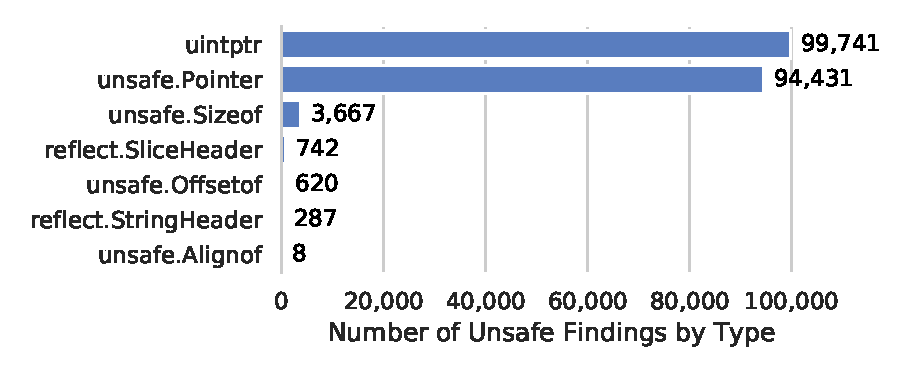
\includegraphics[width=0.43\textwidth]{assets/plots/distribution-unsafe-types.pdf}
    \caption{Distribution of different types of unsafe tokens}
    \label{fig:unsafe-tokens-distribution}
\end{figure}

The data shows that \textit{uintptr} is the most common \unsafe{} token, with \checkNum{99,741} findings.
Next, \textit{unsafe.Pointer} has a similarly high prevalence of \checkNum{94,431} samples.
These two lead the usage counts by far, with the next being \textit{unsafe.Sizeof} at only \checkNum{3,667} usages and
all other token types found less than \checkNum{1,000} times.
With a mere \checkNum{8} usages found, \textit{unsafe.Alignof} is the most rare.

\begin{tcolorbox}[boxsep=3pt, enlarge top by=5pt, title=Answer to~\ref{rq:distTypes}]
    In the wild, uintptr and unsafe.Pointer are orders of magnitude more common than other unsafe usages.
\end{tcolorbox}


%% ---------------------------------------------------------------------------------------------------------------------

\subsection{Influence of Age and Popularity}\label{subsec:go-geiger:evaluation:popularity}

This subsection answers research question~\ref{rq:popularity} about whether there is a correlation between \unsafe{}
usage and the common projects metrics age and popularity.
Popularity is measured by the number of stars and number of forks that a project has on \github{}.
Figure~\ref{fig:correlation-popularity} presents a scatter plot showing the number of \unsafe{} usages on the x-axis and
multiple project metrics on the y-axis.
Each dot represents one project.
Red dots indicate a project's age, blue dots show the number of stars, and green dots denote the number of forks.

\begin{figure}[htp!]
    %\vspace{2mm}
    \centering
    \includegraphics[width=\textwidth]{assets/plots/chapter4/unsafe-import-depth.pdf}
    \caption{TODO: Correlation between \unsafe{} usage and project metrics age and popularity}
    \label{fig:correlation-popularity}
    %\vspace{-10pt}
\end{figure}


The plot suggests that there is no correlation between either age, number of stars, nor number of forks and the number
of \unsafe{} usages in a project.

\begin{tcolorbox}[boxsep=3pt, enlarge top by=5pt, title=Answer to~\ref{rq:popularity}]
    There is no significant correlation between the number of \unsafe{} usages and a project's age, number of stars, or
    number of forks.
\end{tcolorbox}


%% ---------------------------------------------------------------------------------------------------------------------

\subsection{Change of Usage over Time}\label{subsec:go-geiger:evaluation:over-time}

The data set collected in this study contains one version of each analyzed project.
Therefore, it is not directly possible to measure the change of \unsafe{} usage in projects over time.
However, there are a number of modules that are included in several versions by different projects, which means these
modules allow an analysis of such changes in \unsafe{} usage.
To answer research question~\ref{rq:changeTime}, this subsection discusses the differences between different version of
an examplary module, \textit{golang.org/x/sys}.

The module is present in the data set with a total of \sysModuleVersions{} versions.
A subset of the versions with a fair distribution of release dates in \checkNum{2019} and \checkNum{2020}, as well as a
rather old version from \checkNum{2017} is shown in Table~\ref{tbl:unsafe-usage-over-time}.
The table shows the version identifiers alongside their release dates and number of \unsafe{} usages in the particular
version.
The module versions are ordered by their release date.

\begin{table}[htp!]
    \centering
    \caption{Change of unsafe usage over time in the golang.org/x/sys module}
    \label{tbl:unsafe-usage-over-time}
    \begin{tabular}{l|l|r}
    \textbf{Version}                   & \textbf{Release date} & \textbf{Unsafe usage count} \\
    \hline
    v0.0.0-20171012164349-43eea11bc926 & 12.10.2017            & 315                         \\
    v0.0.0-20190502145724-3ef323f4f1fd & 02.05.2019            & 387                         \\
    v0.0.0-20190726091711-fc99dfbffb4e & 26.07.2019            & 392                         \\
    v0.0.0-20191001151750-bb3f8db39f24 & 01.10.2019            & 403                         \\
    v0.0.0-20191128015809-6d18c012aee9 & 28.11.2019            & 403                         \\
    v0.0.0-20200107162124-548cf772de50 & 07.01.2020            & 428                         \\
    v0.0.0-20200302150141-5c8b2ff67527 & 02.03.2020            & 428                         \\
    v0.0.0-20200413165638-669c56c373c4 & 13.04.2020            & 434                         \\
    v0.0.0-20200501145240-bc7a7d42d5c3 & 01.05.2020            & 440                         \\
    \end{tabular}
\end{table}

It is evident that there is a monotonous increase in \unsafe{} usage, with an increase from \sysModuleLeastUnsafe{} to
\sysModuleMostUnsafe{} (\sysModuleUnsafeIncrease) over the \checkNum{2.5 years} period from \checkNum{2017} to
\checkNum{2020}.
A manual analysis of the changes in the module source code shows that the increased usages of \unsafe{} in this case are
caused by additional system call \acrshort{API}s that are supported by the module.
Dispatching to the underlying system call code requires the use of \textit{unsafe.Pointer}.
Therefore, in this case more features provided by a dependency cause more \unsafe{} code to be imported into a project.

\begin{tcolorbox}[boxsep=3pt, enlarge top by=5pt, title=Answer to~\ref{rq:changeTime}]
    Changes in \unsafe{} usage in particular modules are motivated for example by new \acrshort{API} requirements and
    can be significant, with e.g. about a \sysModuleUnsafeIncreaseRounded{} increase found in the
    \textit{sys} module.
\end{tcolorbox}


%% ---------------------------------------------------------------------------------------------------------------------

\subsection{Comparison with Existing Tools}\label{subsec:go-geiger:evaluation:linters-comparison}

To evaluate the benefit \toolGeiger{} provides in comparison to existing linters for Go, its findings are put in context
with the results of \toolVet{} and \toolGosec{} in this section.
The goal of this comparison is to see whether any of those tools can achieve the same as \toolGeiger{} does.
As described in Section~\ref{sec:background:static-code-analysis}, \toolVet{} is a linter that is included as part of
the standard Go command line tool chain.
It runs a number of analysis passes to identify general problems with the source code.
There is the \textit{unsafeptr} pass, which is designed to find potential misuses of the \textit{unsafe.Pointer} type.
It is however not designed for a general identification of \unsafe{} usages.
On the other hand, \toolGosec{} is a static analysis tool with a design focused around security problems.
It is built from several rules to identify issues, one of which (\textit{\checkNum{G103}}) is simply triggered by the
presence of \unsafe{} package members and generates a warning that those usages should be audited.
Given this design, it is closer to \toolGeiger{} in the sense that it only identifies the presence of \unsafe{} without
using any logic to determine potential misuses.

To conduct the comparison, \toolVet{} and \toolGosec{} are run on the same \packagesAnalyzed{} packages that were
analyzed with \toolGeiger{}.
The results are part of the data set as well.
Then, the findings of the tools are matched using package, file name, and line number information.
Table~\ref{tbl:go-geiger-evaluation-linters} shows the results of this analysis.
The result columns are divided to show the different results for \toolVet{} and \toolGosec{}.
True positives (TP) are lines of code that were both flagged by \toolGeiger{} and the respective linter tool.
False negatives (FN) denote lines that were only flagged by \toolGeiger{}, but not by the linter.
Finally, false positives (FP) indicate that the linter flagged a line that was not identified by \toolGeiger{}.
There is no column for true negatives because the number of these is irrelevant for this analysis.
The table contains two rows that show the number of lines of code both when counting any message that \toolVet{} or
\toolGosec{} produced and when only messages related to their \unsafe{} analyses are taken into account.
The latter has more impact because comparing only those messages to the output of \toolGeiger{}, which is solely
designed around \unsafe{} usages, achieves a fairer evaluation.

\begin{table}[htp!]
    \centering
    \caption{Comparison of the performances of \toolGeiger{} and other linters}
    \label{tbl:go-geiger-evaluation-linters}
    \begin{tabular}{l|rr|rr|rr}
        \textbf{Scenario} & \multicolumn{2}{c|}{\textbf{TP (both)}} & \multicolumn{2}{c|}{\textbf{FN (only \toolGeiger{})}} & \multicolumn{2}{c}{\textbf{FP (only linter)}} \\
        {}                & go vet    & gosec              & go vet          & gosec                      & go vet      & gosec                  \\
        \hline
        Any message       & 219       & 36,279             & 76,738          & 40,678                     &  31,224     & 114,306                \\
        Related message   & 213       & 26,267             & 76,744          & 18,019                     &       0     & 0                      \\
    \end{tabular}
\end{table}

The results show that there is only a very small number of true positives for \toolVet{}, but many false negatives.
This means that for most of the \unsafe{} usages \toolVet{} does not generate a warning.
When comparing any message generated by \toolVet{}, there are many false positives, however those do not exist anymore
when the analysis is restricted to \toolVet{} messages related to \unsafe{}.
This means that while \toolVet{} provides a lot of warnings that are related to other problems, it does not offer any
benefit over \toolGeiger{} for the specific task of identifying \unsafe{} usages.
For \toolGosec{}, there are a lot more true positives, but still a lot of false negatives.
About \checkNum{half} of the \toolGeiger{} results are also found by \toolGosec{}.
This is much better than \toolVet{}, but it is still not accurate.
One reason for this is that \toolGeiger{} identifies not only \textit{unsafe} packages uses, but also \textit{uintptr}
which is common as described in Section~\ref{subsec:go-geiger:evaluation:unsafe-usage}.
Similar to \toolVet{}, there are many false positives when any \toolGosec{} message is counted, but there are none when
only \unsafe{}-related messages are analyzed.
Therefore, \toolGosec{} can not detect any usages that \toolGeiger{} would miss.
It is worth noting that the numbers in Table~\ref{tbl:go-geiger-evaluation-linters} refer to lines of code rather than
\unsafe{} findings, but one line of code can contain several \unsafe{} usages.
Therefore the numbers do not add up to the same total findings discussed in
Section~\ref{subsec:go-geiger:evaluation:unsafe-usage}.

\begin{tcolorbox}[boxsep=3pt, enlarge top by=5pt, title=Answer to~\ref{rq:linterComparison}]
    The existing tools \toolVet{} and \toolGosec{} do not provide any benefit over \toolGeiger{} for the specific task
    it is designed for.
    Instead, \toolGeiger{} finds all and more of their \unsafe{}-related results.
\end{tcolorbox}


%% ---------------------------------------------------------------------------------------------------------------------

\section{Purpose of Unsafe in Practice: a Labeled Data Set}\label{sec:go-geiger:labeled-dataset}

This chapter presents an in-depth study of the purpose of \unsafe{} usages in \projsForLabeledCodeSnippets{} selected
open-source Go projects.
The result of this is a manually labeled data set of \numberLabeledCodeSnippets{} code samples.
It is available online in the same data repository as the study results presented in the previous section.
These samples are divided into \numberLabeledCodeSnippetsStd{} standard library samples (\textit{std}) and
\numberLabeledCodeSnippetsApp{} non-standard-library application samples (\textit{app}).
The purpose of this data set is to understand what operations are done in practice using the \unsafe{} \acrshort{API},
and for what purpose.
Thus, each sample is labeled in two dimensions by the operation type and its higher-level goal.
The \numberLabeledCodeSnippets{} code samples are drawn from the projects listed in Table~\ref{tbl:dataset-projects}.

\begin{table}[!t]
\vspace{2mm}

    \centering
    \caption{Projects selected for labeled data set}
    \label{tbl:dataset-projects}
    \begin{adjustbox}{max width=\textwidth}
    \begin{tabular}{llrrl}
        %\hline
        {} & \textbf{Name} &  \textbf{Stars} &  \textbf{Forks} &    \textbf{Revision} \\ \hline
        \rowcolor{verylightgray}
        1  &         kubernetes/kubernetes &  66,512 &  23,806 &  \texttt{fb9e1946b0} \\
        2  &                 elastic/beats &   8,852 &   3,207 &  \texttt{df6f2169c5} \\
        \rowcolor{verylightgray}
        3  &             gorgonia/gorgonia &   3,373 &    301 &  \texttt{5fb5944d4a} \\
        4  &              weaveworks/scope &   4,354 &    554 &  \texttt{bf90d56f0c} \\
        \rowcolor{verylightgray}
        5  &  mattermost/mattermost-server &  18,277 &   4,157 &  \texttt{e83cc7357c} \\
        6  &               rancher/rancher &  14,344 &   1,758 &  \texttt{56a464049e} \\
        \rowcolor{verylightgray}
        7  &                 cilium/cilium &   5,501 &    626 &  \texttt{9b0ae85b5f} \\
        8  &                     rook/rook &   7,208 &   1,472 &  \texttt{ff90fa7098} \\
        \rowcolor{verylightgray}
        9  &             containers/libpod &   4,549 &    539 &  \texttt{e8818ced80} \\
        10 &                       xo/usql &   5,871 &    195 &  \texttt{bdff722f7b} \\ %\hline
    \end{tabular}
    \end{adjustbox}
    %% reduce space after table for vspace tweaking
    \vspace{-10pt}
\end{table}

They were selected based on their high number of \unsafe{} usages, and taking care that they represent a reasonably
large diversity.
The projects contain applications based around containers and operations, chat, infrastructure as a service, data
storage, visualization, and machine learning.
When selecting samples to look at, I deliberately separated the standard library from application usages.
This decision is based on the results presented in Section~\ref{subsec:go-geiger:evaluation:unsafe-usage}, which show
that all projects must use the standard library, as well as the hypothesis that the standard library uses different
\unsafe{} patterns.

Standard library is defined by the packages that live in the Go \textit{std} and the \texttt{golang.org/x/sys} module.
The \textit{sys} module is included because it contains a lot of system call infrastructure and is the replacement for
the deprecated \textit{syscall} package\footnote{\url{https://golang.org/pkg/syscall}}.
Thus, it is also maintained by the core Go developer team.
Application code samples then are taken from packages that are not part of the standard library.
The \numberLabeledCodeSnippets{} code examples were sampled randomly from all packages present in the dependency trees
of the projects shown in Table~\ref{tbl:dataset-projects}.
This increases the variety of code authors contributing to the code examples.
However, they are taken without duplicating lines that are present in different versions of the same module.
If a module is included in multiple versions, than a line of code within it can not be drawn twice from differnt
versions.
Furthermore, this labeled data set contains only usages of \textit{unsafe.Pointer}.

Listing~\ref{lst:dataset-label-class-examples} shows code examples and descriptions for each of the classes used to
describe what is happening in an unsafe usage.
Each example also contains its respective purpose label.

\begin{lstlisting}[language=Golang, label=lst:dataset-label-class-examples, caption=Example code snippets for different classes in the data set]
// cast-basic, efficiency
out = (*int32)(unsafe.Pointer(in))

// cast-bytes, serialization
return (*(*[10]byte)(unsafe.Pointer(x)))[:]

// cast-header, efficiency
hdr := &reflect.SliceHeader{
    Data: uintptr(unsafe.Pointer(&data[i])),
    Len:  42,
    Cap:  42,
}
retVal = append(retVal, *(*[]uint8)(unsafe.Pointer(hdr)))

// cast-pointer, serialization
return unsafe.Pointer(ptr)

// cast-struct, efficiency
out = (*runtime.Unknown)(unsafe.Pointer(in))

// definition, serialization
type unsafeType struct {
    ptr unsafe.Pointer
}

// delegate, serialization
func (encoder *dynamicEncoder) Encode(ptr unsafe.Pointer) {
    encoder.UnsafeIndirect(ptr)
}

// memory-access, serialization
deReferenced := *((*unsafe.Pointer)(ptr))

// pointer-arithmetic, layout
unaligned := uintptr(unsafe.Pointer(&value[0])) & 3

// syscall, no-gc
n, _, errno := syscall.Syscall(syscall.SYS_RECVMSG, s,
    uintptr(unsafe.Pointer(h)), uintptr(flags))

// unused, unused
func Encode(ptr unsafe.Pointer, stream *Stream) {
    stream.WriteEmptyArray()
}
\end{lstlisting}

The classes are outlined briefly in the following paragraphs.
For the \unsafe{} operation type dimension, the most common labels are conversions between types.
The \textit{cast-struct}, \textit{cast-basic}, \textit{cast-header}, \textit{cast-bytes}, and \textit{cast-pointer}
classes represent conversions between arbitrary types, where one of them is a structure, a basic type such as
\textit{int}, a slice or string header structure, a \textit{[]byte} array, or \textit{unsafe.Pointer} directly,
respectively.
The \textit{memory-access} class is used where unsafe.Pointer values are dereferenced, used to manipulate corresponding
memory or for comparison with another address.
\textit{Pointer-arithmetic} is a class containing any form of arithmetic address manipulation such as advancing an
array.
The \textit{definition} class denotes usages where a field or method of type \textit{unsafe.Pointer} is declared for
later usage.
When \unsafe{} is only required to pass it along to another function that expects a parameter of type
\textit{unsafe.Pointer}, the \textit{delegate} label is applied.
Thus, for this class the need for \unsafe{} is at a different location in the code.
\textit{Syscall} represents calls using the Go \textit{syscall} package or \textit{golang.org/x/sys} module.
Finally, \textit{unused} contains instances of \unsafe{} that are not actually used in the analyzed code, such as dead
code or unused parameters.

In the purpose dimension, the \textit{efficiency} class represents cases where unsafe is used only to improve time or
space efficiency of the code.
Usages in this class could be rewritten to not use \unsafe{}.
The \textit{serialization} class includes (un)marshalling and (de)serialization operations like in-place casts between
complex types and bytes.
\textit{Generics} is used where \unsafe{} is used to build functionality that would be implemented using generics if
they were available in Go.
The \textit{avoid garbage collection} class contains usages to ask the Go compiler to not free a value while it is used,
for example by a function written in assembly.
\textit{Atomic operations} is a class of usages of the atomic \acrshort{API}, which requires \unsafe{} for some of its
functions.
The \textit{foreign function interface} (\acrshort{FFI}) class includes all cases of interoperability with C code (CGo),
as well as calls to functions that receive their parameters as unsafe pointers.
\textit{Hide from escape analysis} contains instances where \unsafe{} is used to deliberately exlude a value from being
seen by the \acrshort{EA} algorithm.
The \textit{memory layout control} class represents code used for low-level memory management.
\textit{Types} samples are used by the standard library for low-level implementation of the Go type system.
\textit{Reflect} includes instances of type reflection, as well as re-implementations of types contained in the regular
Go \textit{reflect} package, for example to use \textit{unsafe.Pointer} instead of \textit{uintptr} for slice headers.
Lastly, \textit{unused} is the class for unused occurrences again.

Table~\ref{tbl:dataset-classes} presents the number of samples for each label.
The columns denote the dimension of purpose, while the rows show the operation type dimension.
Columns are divided into separate counts for the \textit{app} and \textit{std} groups of samples.

\begin{table*}[htp!]
    \centering
    \caption[Labeled unsafe.Pointer usages in application code (non standard library) and standard library samples]
        {Labeled unsafe.Pointer usages in application code (non standard library) and standard library samples~\newline \tiny ~\newline \footnotesize
        \underline{eff}: efficiency, \underline{ser}: (de)serialization, \underline{gen}: generics,
        \underline{no GC}: avoid garbage collection, \underline{atomic}: atomic operations,
        \underline{FFI}: foreign function interface, \underline{HE}: hide from escape analysis, \underline{layout}: memory layout control,
        \underline{types}: Go type system,
        \underline{reflect}: type reflection, \underline{unused}: declared but unused \tiny ~\newline}
    \label{tbl:dataset-classes}
    \begin{adjustbox}{max width=\textwidth}
    
    %% do not paste from notebook, local changes done!
\begin{tabular}{r|cc|cc|cc|cc|cc|cc|cc|cc|cc|cc|cc|cc}
                    & \multicolumn{2}{c|}{\textbf{eff}} & \multicolumn{2}{c|}{\textbf{ser}} & \multicolumn{2}{c|}{\textbf{gen}} & \multicolumn{2}{c|}{\textbf{no GC}} & \multicolumn{2}{c|}{\textbf{atomic}} & \multicolumn{2}{c|}{\textbf{FFI}} & \multicolumn{2}{c|}{\textbf{HE}} & \multicolumn{2}{c|}{\textbf{layout}} & \multicolumn{2}{c|}{\textbf{types}} & \multicolumn{2}{c|}{\textbf{reflect}} & \multicolumn{2}{c|}{\textbf{unused}} & \multicolumn{2}{c}{\textbf{Total}} \\ %\hline
                    &  \textbf{app} &  \textbf{std} &  \textbf{app} &  \textbf{std} &  \textbf{app} &  \textbf{std} &   \textbf{app} &  \textbf{std} &    \textbf{app} &  \textbf{std} &  \textbf{app} &  \textbf{std} &  \textbf{app} &  \textbf{std} &    \textbf{app} &  \textbf{std} &   \textbf{app} &  \textbf{std} &     \textbf{app} &  \textbf{std} &    \textbf{app} &  \textbf{std} &   \textbf{app} &  \textbf{std} \\ \hline
                    
                   % \textbf{cast} & 562 & 16 & 178 & 33 & 18 & & & & & & 24 & 6 && 2 & 3 & 13 & & 45 & 1 & & & & 786 & 115 \\
        \textbf{cast-struct} &  401 &    4 &   50 &    6 &    6 &      &       &      &        &      &    6 &    2 &      &    2 &        &    4 &       &   31 &         &      &        &      &   463 &   49 \\
\rowcolor{verylightgray}
         \textbf{cast-basic} &   90 &    2 &   29 &    3 &    1 &      &       &      &        &      &    1 &    3 &      &      &      2 &    7 &       &    1 &         &      &        &      &   123 &   16 \\
                    \textbf{cast-header} &   36 &    1 &    3 &      &    1 &      &       &      &        &      &      &      &      &      &        &      &       &    3 &         &      &        &      &    40 &    4 \\
\rowcolor{verylightgray}
                    \textbf{cast-bytes} &   22 &    1 &   81 &   11 &      &      &       &      &        &      &    1 &      &      &      &      1 &      &       &    1 &         &      &        &      &   105 &   13 \\
                    \textbf{cast-pointer} &   13 &    8 &   15 &   13 &   10 &      &       &      &        &      &   16 &    1 &      &      &        &    2 &       &    9 &       1 &      &        &      &    55 &   33 \\
\rowcolor{verylightgray}
      \textbf{memory-access} &    2 &    1 &    9 &      &      &      &       &      &        &      &      &    1 &      &      &      4 &    6 &       &    4 &         &      &        &      &    15 &   12 \\
 \textbf{pointer-arithmetic} &    7 &    2 &    6 &    1 &      &      &       &      &        &    1 &      &    3 &    1 &    2 &      3 &    8 &       &    9 &         &      &        &      &    17 &   26 \\
\rowcolor{verylightgray}
         \textbf{definition} &    4 &    1 &   23 &      &    2 &      &       &      &        &      &    4 &    5 &      &      &        &    9 &       &    8 &       6 &    3 &        &      &    39 &   26 \\
           \textbf{delegate} &    4 &      &   64 &      &    2 &      &       &      &     11 &    5 &   29 &   45 &      &    4 &        &   14 &       &    6 &         &    1 &        &      &   110 &   75 \\
\rowcolor{verylightgray}
            \textbf{syscall} &      &      &      &      &      &      &    17 &  138 &        &      &      &      &      &      &        &      &       &      &         &      &        &      &    17 &  138 \\
             \textbf{unused} &      &      &      &      &      &      &       &      &        &      &      &      &      &      &        &      &       &      &         &      &     16 &    8 &    16 &    8 \\ \hline
%\rowcolor{verylightgray}
                  \textbf{total} &  579 &   20 &  280 &   34 &   22 &    0 &    17 &  138 &     11 &    6 &   57 &   60 &    1 &    8 &     10 &   50 &     0 &   72 &       7 &    4 &     16 &    8 &  1000 &  400 \\
\end{tabular}

    \end{adjustbox}
        \vspace{-10pt}
\end{table*}

The data shows that efficiency is by far the most prevalent reason to use \unsafe{} code in real-world Go application
code.
While the usages in \textit{cast} classes make up about \checkNum{58\%} of the application code samples, only about
\checkNum{5\%} of the standard library usages are for efficiency.
Within the \textit{efficiency} class, casting operation cover most of the usages with \checkNum{97\%} (\textit{app}) and
\checkNum{80\%} (\textit{std}) of the samples.
Next, the second most important motivation for \unsafe{} code in the application class is performing serialization or
deserialization operations, including marshalling of structured data to interchangeable formats.
This accounts for \checkNum{28\%} of the usages.
The standard library shows a different most common usage, which is avoiding garbage collection with \checkNum{25\%}.
This purpose is only found in \checkNum{2\%} of the \textit{app} samples.
Next, the \textit{type} (\checkNum{18\%}), \textit{\acrshort{FFI}} (\checkNum{15\%}), and \textit{memory layout}
(\checkNum{13\%}) classes are common in the \textit{std} samples.
A common distribution is the hiding from escape analysis class, which is rare both in the \textit{app}
(\checkNum{0.1\%}) and \textit{std} (\checkNum{2\%}) groups.
The same is true for the \textit{reflection} class (\checkNum{1\%} in both sets).
There are also only few samples (\checkNum{2\%}) that are used to implement generics functionality, which is not
available in current versions of Go.
Some of the findings in the \textit{serialization} class could however be achieved with generics as well, so the classes
overlap slightly.

\begin{tcolorbox}[boxsep=3pt, enlarge top by=5pt, title=Answer to~\ref{rq:purpose}]
    \checkNum{More than half} of the \unsafe{} usages in projects and 3rd party libraries are to improve efficiency via
    \unsafe{} casts.
    In the Go standard library, \checkNum{every third} use of \unsafe{} is to avoid garbage collection.
\end{tcolorbox}
